\documentclass[handout]{ximera}
\input{../../preamble}

\title{Review of integration}

\begin{document}
\begin{abstract}
We review indefinite and definite integration from Calc 1
\end{abstract}
\maketitle

\begin{center}
\large{\textbf{Welcome to MTH 182!}}
\end{center}

 Today we are reviewing integration.  You will be reviewing how to \textbf{calculate} integrals in your WebWork.  This class period will be devoted to a review of the \textbf{concepts} of integral calculus (which is just as, if not more, important for your success in this class than the calculations).
 
\begin{exercise}
	
	Having contact information for at least one or two classmates will be very valuable to you if you miss a class, or want some quick input from a fellow student.
	
   	Find two other people sitting near you.  If they feel comfortable giving you this information, record their name, phone number and email address.
   	
   	Person 1:

	Person 2:
	

\end{exercise}


 
 Recall the following definition:
 
\begin{definition}
		Let $f$ be a function defined on an interval $(a,b)$.  Then an \textbf{antiderivative} of $f$ is a function $F$ such that 
		
		\begin{center}$\rule{3 in}{0.15mm}$ for all $x \in (a,b)$
		\end{center}
\end{definition}

\begin{question}
	Which of the following are antiderivatives of $\frac{1}{x\ln(x^2)}$ (There could be more than one)?
	\begin{selectAll}
		\choice[correct]{$\ln(x^2)$}
		\choice[correct]{$\frac{\ln(2) + \ln(\ln(x))}{2}$}
		\choice[correct]{$\frac{\ln(\ln(x^3))}{2}$}
	\end{selectAll}
\end{question}
 
\begin{exercise}
	
	The graph of a function $f$ is shown below.  Sketch two \textbf{different} antiderivatives of $f$ on the same set of axes.
	
\begin{image}
	\begin{tikzpicture}
	\begin{axis}[
	domain=-5:5, ymax=10,xmax=4,ymin=-5, xmin=-4,
	axis lines =center, xlabel=$x$, ylabel=$y$,
	ticks=none,
	every axis y label/.style={at=(current axis.above origin),anchor=south},
	every axis x label/.style={at=(current axis.right of origin),anchor=west},
	axis on top,
	]

	\addplot [draw=penColor,very thick] {(x+1)*(x-2)};
    \node at (axis cs:3,7) [penColor] {$f$};

	
	\end{axis}
	\end{tikzpicture}
\end{image}

What do you notice about these two antiderivatives?

\end{exercise}

Recall the following ``definition'':

\begin{definition}\index{integral}\index{definite integral}
	The \dfn{definite integral}
	\[
	\int_a^b f(x) \d x
	\]
	computes the signed area between $y=f(x)$ and the $x$-axis on the
	interval $[a,b]$.
	\begin{itemize}
		\item If the region is above the $x$-axis, then the area has
		positive sign.
		\item If the region is below the $x$-axis, then the area has
		negative sign.
	\end{itemize}
	Note, when working with signed area, ``positive'' and ``negative''
	area cancel each other out.
\end{definition}


It will also be useful to adopt the following intuitive way of
thinking about this definite integrals: we can
think of an integral as ``summing up" an infinite number of
infinitesimal quantities. In this case we are summing rectangles of
width $\d x$ and height $f(x)$:

\begin{image}
	\begin{tikzpicture}
	\begin{axis}[
	domain=-0.5:2.5, ymax=10,xmax=2.5,ymin=-1, xmin=-0.5,
	axis lines =center, xlabel=$x$, ylabel=$y$,
	xtick={1,2}, yticklabels={},
	ytick style={draw=none},
	xticklabels={$a$, $b$},
	width=4in,
	height=2in,
	every axis y label/.style={at=(current axis.above origin),anchor=south},
	every axis x label/.style={at=(current axis.right of origin),anchor=west},
	axis on top,
	]
	%\addplot [draw=none,fill=fillp,domain=1:2] {-x^2+4*x+3} \closedcycle;
	%\addplot [draw=none,fill=background,domain=1:2] {-x^3 + 7*x^2-10*x+5} \closedcycle;
	\addplot [draw=penColor,very thick] {-x^2+4*x+3};
	%\addplot [draw=penColor2,very thick] {-x^3 + 7*x^2-10*x+5};
	\node at (axis cs:1,6.7) [penColor] {$f$};
%	\node at (axis cs:2,4) [penColor2] {$g$};
	\addplot [draw=penColor, fill = fillp] plot coordinates {(1.5,0) (1.6,0) (1.6, 6.84) (1.5,6.84) (1.5, 0)};
	

	
	\node at (axis cs:1.55,-0.5) {$\d x$};
	
	\draw[decoration={brace,raise=.2cm},decorate,thin] (axis cs:1.51,0)--(axis cs:1.51,6.84);
	\node[anchor=east] at (axis cs:1.45,3.4) {$f(x)$};
	\end{axis}
	\end{tikzpicture}
\end{image}
In this case, the integral
\begin{image}
	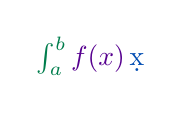
\begin{tikzpicture}[scale=1,every node/.style={transform shape}]
	\node at (0,0) {
		$\color{green!70!black!70!blue}\int_{a}^{b}\color{purple!50!blue!90!black}{f(x)} \,\color{blue!70!green}{\d x}$
	};
	\end{tikzpicture}
\end{image}
could be interpreted as:
\begin{quote}
	\large\textbf{The \textcolor{green!70!black!70!blue}{sum} of the
		area of rectangles whose
		\textcolor{purple!50!blue!90!black}{heights are given by $f$}, and whose
		\textcolor{blue!70!green}{widths are infinitesimal}.}
\end{quote}

\begin{question}
	Consider the following graph of $y=f(x)$:
	\begin{image}
		\begin{tikzpicture}
		\begin{axis}[
		width=6in,
		height=3in,
		xmin=-.5, xmax=5.5,ymin=-1.2,ymax=1.2,domain=0:6,
		axis lines =center, xlabel=$x$, ylabel=$y$,
		every axis y label/.style={at=(current axis.above origin),anchor=south},
		every axis x label/.style={at=(current axis.right of origin),anchor=west},
		axis on top,
		] 
		\addplot [draw=none, %pattern=north west lines, pattern color=blue,
		fill=fillp,
		domain=0:1] {x} \closedcycle;
		\addplot [draw=none, %pattern=north west lines, pattern color=blue,
		fill=fillp,
		domain=1:5] {1.5-x/2} \closedcycle;
		
		\addplot [penColor,very thick,domain=0:1] {x};
		\addplot [penColor,very thick,domain=1:5] {1.5-x/2};
		\end{axis}
		\end{tikzpicture}
	\end{image}
	Compute:


		 \[
		 \int_0^5 f(x) \d x \begin{prompt}= \answer{0.5}\end{prompt}
		 \]


\end{question}

It happens \textbf{very frequently} that we want to consider ``integral valued functions''.  For example

\begin{question}
	
	Let $f(t) = \sqrt{1-t^2}$.  Then the graph of $f$ is the upper half of the unit circle.
	
	Define a new function $A$ by
	
	\[
	A(x) = \int_0^x \sqrt{1-t^2} \d t
	\]
	
\begin{image}
	\begin{tikzpicture}
	\begin{axis}[
	xmin=-1.1,xmax=1.1,ymin=-1.1,ymax=1.1,
	axis lines=center,
	width=4in,
	xtick={-1,1},
	ytick={-1,1},
	clip=false,
	%unit vector ratio*=1 1 1,
	xlabel=$t$, ylabel=$y$,
	every axis y label/.style={at=(current axis.above origin),anchor=south},
	every axis x label/.style={at=(current axis.right of origin),anchor=west},
	]        
	\addplot [smooth, domain=(0:180)] ({cos(x)},{sin(x)});
	\addplot [fill=fillp, domain=(0:0.5)] {sqrt(1-x^2)}\closedcycle;
	\node at (axis cs:0.5,-0.1) [textColor] {$x$};
	\node at (axis cs:0.25,0.4) [textColor] {\[A(x)\]};

	 %% unit circle
	

	\end{axis}
	\end{tikzpicture}
\end{image}



	
	Then
	
	\[A(0) = \]
	\[A(1) = \]
	\[A(-1)=\]
	
	Sketch a graph of $A$:
	
\begin{image}
	\begin{tikzpicture}
	\begin{axis}[
	xmin=-1.1,xmax=1.1,ymin=-3,ymax=3,
	axis lines=center,
	width=4in,
	xtick={-1,1},
	%ytick={-1,1},
	clip=false,
	xlabel=$t$, ylabel=$y$,
	every axis y label/.style={at=(current axis.above origin),anchor=south},
	every axis x label/.style={at=(current axis.right of origin),anchor=west},
	]        
	
	
	\end{axis}
	\end{tikzpicture}
\end{image}

\textbf{Challenge:}  Can you find a formula for $A(x)$ using geometry?  This is challenging, but doable.  If you can do it I will be super impressed.

\end{question}

\begin{question}
	Remember that function from \textbf{Question 2}?
	
	I have reproduced its graph below.
	
	Sketch graphs of the following two functions:
	
		\[
		A(x) = \int_0^x f(t) \d t
		\] 
		
		\[
		B(x) = \int_1^x f(t) \d t
		\] 
	
	\begin{image}
		\begin{tikzpicture}
		\begin{axis}[
		domain=-5:5, ymax=10,xmax=4,ymin=-5, xmin=-4,
		axis lines =center, xlabel=$x$, ylabel=$y$,
		ticks=none,
		every axis y label/.style={at=(current axis.above origin),anchor=south},
		every axis x label/.style={at=(current axis.right of origin),anchor=west},
		axis on top,
		]
		
		\addplot [draw=penColor,very thick] {(x+1)*(x-2)};
		\node at (axis cs:3,7) [penColor] {$f$};
		
		
		\end{axis}
		\end{tikzpicture}
	\end{image}
	
	What do you notice about these two functions? How do they compare to the antiderivatives we sketched in question $2$?
	
\end{question}

The answer to the previos question should remind you of the following two theorems:

\begin{theorem}[First Fundamental Theorem of Calculus]\index{First Fundamental Theorem of Calculus}
	Suppose that $f$ is continuous on the real numbers and let
	\[
	F(x)=\int_a^x f(t)\d t.
	\]
	Then $F'(x)=f(x)$.
\end{theorem}
The First Fundamental Theorem of Calculus says that an accumulation
function of $f$ is an antiderivative of $f$. Another way of saying
this is:
\begin{image}
	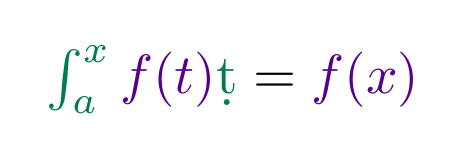
\begin{tikzpicture}[scale=2,every node/.style={transform shape}]
	\node at (0,0) {
		$\color{blue!70!green}\ddx \color{green!70!black!70!blue}\int_a^x\color{purple!50!blue!90!black}f(t)\color{green!70!black!70!blue}\d t\color{black} = \color{purple!50!blue!90!black}f(x)$
	};
	\end{tikzpicture}
\end{image}
This could be read as:%%BADBAD I want this all in bold and with colors
\begin{quote}\large\textbf{The \textcolor{blue!70!green}{rate} that \textcolor{green!70!black!70!blue}{accumulated area} under a  \textcolor{purple!50!blue!90!black}{curve} grows is described identically by that  \color{purple!50!blue!90!black}{curve}.}
\end{quote}


\begin{theorem}[Second Fundamental Theorem of Calculus]\index{Second Fundamental Theorem of Calculus}
	Let $f$ be continuous on $[a,b]$. If $F$ is \textbf{any}
	antiderivative of $f$, then
	\[
	\int_a^b f(x)\d x = F(b)-F(a).
	\]

\end{theorem}

We could rewrite this in an equilvent form (why is it equivalent?):


\begin{image}
	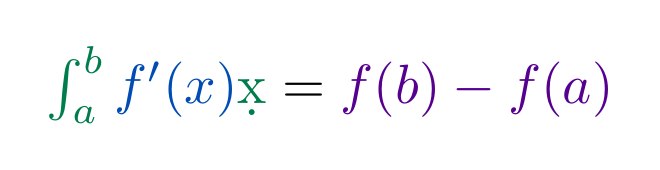
\begin{tikzpicture}[scale=2,every node/.style={transform shape}]
	\node at (0,0) {
		$\color{green!70!black!70!blue}\int_a^b\color{blue!70!green}f'(x)\color{green!70!black!70!blue}\d x\color{black} = 
		\color{purple!50!blue!90!black}f(b) - f(a)$
	};
	\end{tikzpicture}
\end{image}
This could be read as:%%BADBAD I want this all in bold and with colors
\begin{quote}\large\textbf{The \textcolor{green!70!black!70!blue}{accumulation} of a \textcolor{blue!70!green}{rate} is given by the \textcolor{purple!50!blue!90!black}{change in the amount}.}
\end{quote}

\textbf{IMPORTANT:} You use the second fundamental theorem of calculus all the time without really thinking about it.  For instance, in the following calculation

\begin{align*}
	\int_1^2 x \d x &= \left. \frac{1}{2}x^2\right|_1^2\\
		&= \frac{1}{2}(2)^2 - \frac{1}{2}(1)^2\\
		&=\frac{3}{2}
\end{align*}

The Second Fundamental Theorem of Calculus is used on the very first line!  We use the theorem to reinterpret a definite integral (an area!) as the difference in values of an antiderivative of the integrand.

\end{document}